%% This is file `DEMO-TUDaBeamer.tex' version 2.09 (2020/03/09),
%% it is part of
%% TUDa-CI -- Corporate Design for TU Darmstadt
%% ----------------------------------------------------------------------------
%%
%%  Copyright (C) 2018--2020 by Marei Peischl <marei@peitex.de>
%%
%% ============================================================================
%% This work may be distributed and/or modified under the
%% conditions of the LaTeX Project Public License, either version 1.3c
%% of this license or (at your option) any later version.
%% The latest version of this license is in
%% http://www.latex-project.org/lppl.txt
%% and version 1.3c or later is part of all distributions of LaTeX
%% version 2008/05/04 or later.
%%
%% This work has the LPPL maintenance status `maintained'.
%%
%% The Current Maintainers of this work are
%%   Marei Peischl <tuda-ci@peitex.de>
%%   Markus Lazanowski <latex@ce.tu-darmstadt.de>
%%
%% The development repository can be found at
%% https://github.com/tudace/tuda_latex_templates
%% Please use the issue tracker for the feedback!
%%
%% ============================================================================
%%
% !TeX program = lualatex
%%

\documentclass[
english,%globale Übergabe der Hauptsprache
aspectratio=169,%Beamer eigene Option zum Umschalten des Formates
color={accentcolor=3b},
logo=true,%Kein Logo auf Folgeseiten
colorframetitle=false,%Akzentfarbe auch im Frametitle
%	logofile=example-image, %Falls die Logo Dateien nicht vorliegen
]{tudabeamer}
\usepackage[main=english]{babel}
\usepackage{xcolor}


\usepackage{tikz, wrapfig}
\graphicspath{{figures/}}
\usepackage{subcaption}
\usepackage{float}
\usepackage{graphicx}
\usetikzlibrary{positioning}
\usetikzlibrary{arrows}

% Der folgende Block ist nur bei pdfTeX auf Versionen vor April 2018 notwendig
\usepackage{iftex}
\ifPDFTeX
\usepackage[utf8]{inputenc}%kompatibilität mit TeX Versionen vor April 2018
\fi


%Makros für Formatierungen der Doku
%Im Allgemeinen nicht notwendig!
\let\code\texttt

\title{Bayesian Inference of Information Transfer in Networked Multi-Agent Systems}
\subtitle{Master-Thesis}
\author[G.Ekinci]{Gizem Ekinci}
\department{BCS, TU Darmstadt}

%Fremdlogo
%Logo Macro mit Sternchen skaliert automatisch, sodass das Logo in die Fußzeile passt
\logo*{
\includegraphics{bcs_logo}}

% Da das Bild frei wählbar nach Breite und/oder Höhe skaliert werden kann, werden \width/\height entsprechend gesetzt. So kann die Fläche optimal gefüllt werden.
%Sternchenversion skaliert automatisch und beschneidet das Bild, um die Fläche zu füllen.

\titlegraphic{}
%\titlegraphic*{\includegraphics{example-image}}
\date{August 21, 2020}

\DeclareRobustCommand{\rchi}{{\mathpalette\irchi\relax}}
\newcommand{\irchi}[2]{\raisebox{\depth}{$#1\chi$}}

\setbeamertemplate{bibliography item}{[\theenumiv]}

\usepackage{algorithmic}
\usepackage[ruled, lined, longend]{algorithm2e}


\begin{document}
	
	\begin{frame}
	\maketitle
	\small
	{\centering\itshape \par}
	\vspace{+4cm}
	\hspace{+10cm}
	Presented by: Gizem Ekinci\par%\medskip
	\begin{tabular}[t]{@{ }l@{\hspace{3pt}}p{.3\textwidth}@{}}
		\hspace{+10cm}
		Supervisors : & Dominik Linzner \\
		& Anam Tahir
	\end{tabular}
\end{frame}


\begin{frame}{Introduction}
\begin{columns}[onlytextwidth,c]
	\column{.8\linewidth}
	\begin{itemize}
		\item Problem: Agent making decisions based on incoming messages, but observes only a summary of them
		\item Objective: To infer this observation model from agent's behaviour
		\item Motivation: Cell to cell communication and cellular decision making \cite{Perkins2009a}
		\begin{itemize}
			\item A cell may emit some message based on its gene activation state. Consider two cells emitting messages, a third cell receiving a translation of these messages. Third cell may have evolved to achieve some task in coordination with other cells.\\
			e.g. the messages containing information about consumption of a particular molecule which needs to be partitioned for survival.
		\end{itemize}
		\item Assuming that the behaviour of agent has been shaped by evolution (close) to optimality
	\end{itemize}
	\column{.2\linewidth}
	%	\begin{wrapfigure}{r}{5cm}
	\centering
	%		\vspace{20pt}
	\resizebox{.85\textwidth}{!}{
		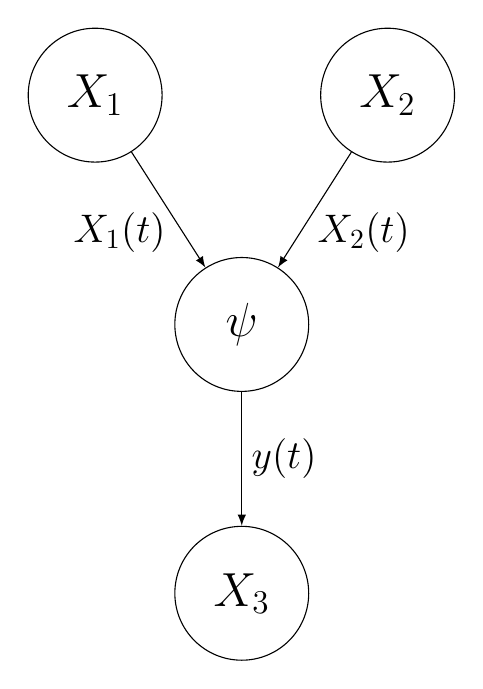
\begin{tikzpicture}
		\tikzstyle{var} = [draw, circle, minimum size=1.7cm]
		\tikzstyle{arrow} = [-latex, line width=0.5pt]
		\tikzstyle{line} = [draw, -latex]
		
		\node [var] (x1) {\LARGE $X_1$};
		\node [var, right=2 cm of x1] (x2) {\LARGE $X_2$};
		\node [var, below right=1.7cm and 0.65cm of x1] (psi) {\LARGE $\psi$};
		\node [var, below=1.7 cm of psi] (x3) {\LARGE $X_3$};
		
		\path [line] (x1)  -- node[pos=0.7, left=.1cm] {\Large$ X_1(t) $} (psi);
		\path [line] (x2)  -- node[pos=0.7, right=.1cm] {\Large$ X_2(t) $} (psi);
		\path [line] (psi)  -- node[midway, right] {\Large$ y(t) $} (x3);
		\end{tikzpicture}
	}
	%		\caption{The communication model.}
	%		\label{fig:graph_model}
	%	\vspace{-8pt}
	%	\end{wrapfigure}
\end{columns}
\end{frame}


\begin{frame}{Problem Formulation}
\framesubtitle{Continuous-time Bayesian network (CTBN)}
% \vspace{-10pt}
\fontsize{9pt}{6}\selectfont
\begin{columns}[onlytextwidth,c]
\column{.2\linewidth}
\centering
\resizebox{.8\textwidth}{!}{
	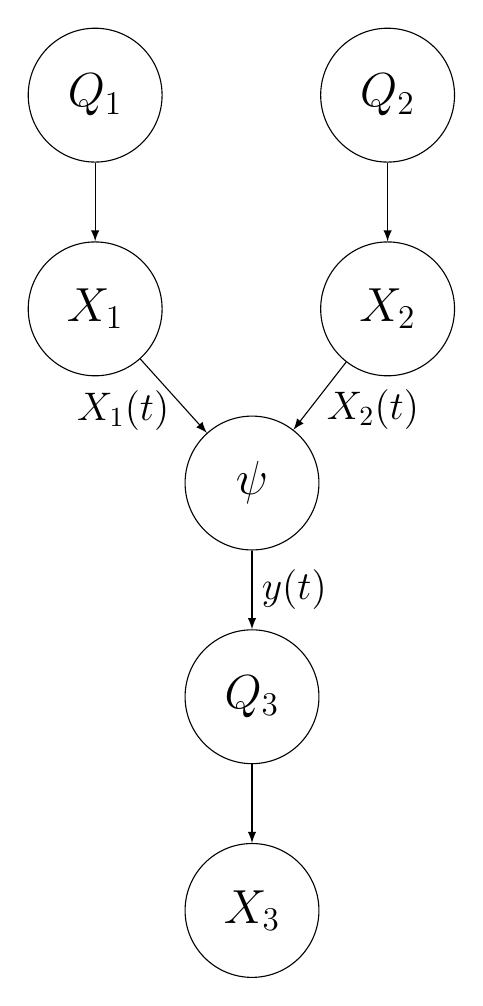
\begin{tikzpicture}
	\tikzstyle{var} = [draw, circle, minimum size=1.7cm]
	\tikzstyle{line} = [draw, -latex]
	
	\node [var] (x1) {\LARGE$X_1$};
	\node [var, above=1cm of x1] (Q1) {\LARGE$ Q_1 $};
	\node [var, right=2cm of x1] (x2) {\LARGE$ X_2 $};
	\node [var, above=1cm of x2] (Q2) {\LARGE$ Q_2 $};
	\node [var, below right=1cm and 0.78cm of x1] (psi) {\LARGE$\psi$};
	\node [var, below=1 cm of psi] (Q3) {\LARGE$Q_3$};
	\node [var, below=1 cm of Q3] (x3) {\LARGE$X_3$};
	
	\path [line] (Q1)  --  (x1);
	\path [line] (Q2)  --  (x2);
	\path [line] (x1)  -- node[pos=0.7, left=.1cm] {\Large$ X_1(t) $} (psi);
	\path [line] (x2)  -- node[pos=0.7, right=.1cm] {\Large$ X_2(t) $} (psi);
	\path [line] (psi)  -- node[midway, right] {\Large$ y(t) $} (Q3);
	\path [line] (Q3)  --  (x3);
	\end{tikzpicture}
}
\column{.8\linewidth}
\begin{itemize}
	\item $ X_{1} $ and $ X_{2} $ homogenous continuous-time Markov processes with $ Q_{1} $ and $ Q_{2} $ transition intensity matrices
	\vspace{-5pt}
	\begin{equation}
	Q_{n} \sim \mathrm{Gam}(\boldsymbol{\alpha}_{n}, \beta_{n})
	\end{equation}
	\item $X_{3} $ conditional continuous-time Markov process  with set of actions $ a \in \left\lbrace a_{0}, a_{1}\right\rbrace  $ and set of transition intensity matrices $ \textbf{\textit{Q}}_{3} = \left\lbrace Q_{3\mid a_{0}}, Q_{3\mid a_{1}} \right\rbrace  $
	%		\vspace{-0.1cm}
	%		\begin{equation}
	%		Q_{a} \sim \mathrm{Gam}(\alpha_{a}, \beta_{a})
	%		\end{equation}
	\item $ X_P $: joint process of $ X_1 $ and $ X_2 $, with factorising state space $ \rchi_{P} = \rchi_1 \times \rchi_2 $
	%		\vspace{-0.1cm}
	%		\begin{equation}
	%			Q_P = Q_{1} * Q_{2}
	%		\end{equation}
	\item Observation model
	\begin{itemize}
		\item $ \psi(x_P) = p(y(t) \mid X_{P}(t)=x_P) $
		\vspace{5pt}
		\item $ \psi $ denoting the matrix with rows $ \left\lbrace \psi(x_P)\right\rbrace_{x_P \in \rchi_P} $
	\end{itemize}
	\item $ \rchi_{n} = \left\lbrace 0,1\right\rbrace $
	\item $ X_{n}^{[0,T]} $: discrete valued trajectory in time interval $ [0, T] $
\end{itemize}
\end{columns}
\end{frame}


\begin{frame}{Problem Formulation}
\framesubtitle{Partially observable Markov decision process (POMDP)}
\vspace{-5pt}
\fontsize{9pt}{6}\selectfont
\centering
\resizebox{.6\textwidth}{!}{
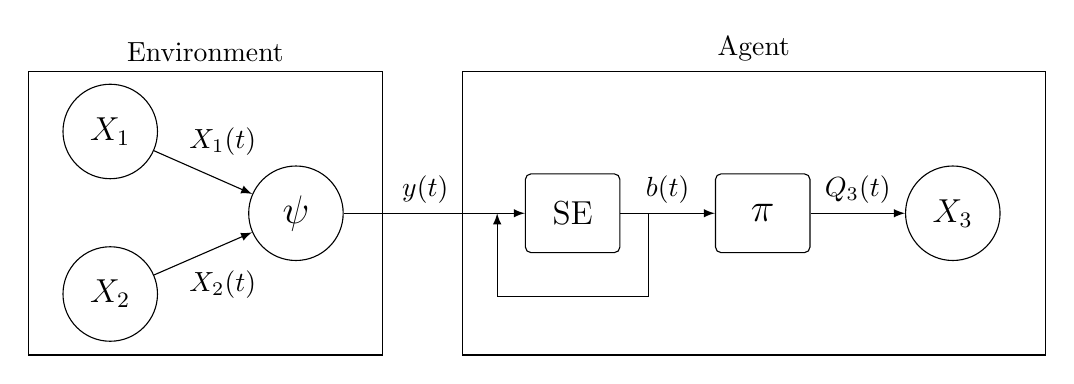
\begin{tikzpicture}
\tikzstyle{var} = [draw, circle, minimum size=1.2cm]
\tikzstyle{vbox} = [draw, rounded corners=2pt, minimum width=1.2cm, minimum height=1cm, align=center]
\tikzstyle{envbox} = [draw, rounded corners=0pt, minimum width=4.5cm, minimum height=3.6cm, align=center]
\tikzstyle{agbox} = [draw, rounded corners=0pt, minimum width=7.4cm, minimum height=3.6cm, align=center]
\tikzstyle{line} = [draw, -latex]

\node [var] (x1) {\large$X_1$};
\node [var, below=0.85cm of x1] (x2) {\large$X_2$};
\node [var, below right=.18cm and 1.5cm of x1] (psi) {\Large$\psi$};
\node [vbox, right=2.3cm of psi] (SE) {\large SE};
\node [vbox, right=1.2cm of SE] (pi) {\Large$ \pi $};
\node [var, right=1.2cm of pi] (x3) {\large$X_3$};
\node [envbox, left=1.8cm of SE] (env) {};
\node [above=0cm of env] {Environment};
\node [agbox, right=1.5cm of psi] (ag) {};
\node [above=0cm of ag] {Agent};

\path [line] (x1)  -- node[pos=0.7, above=.2cm] {$ X_1(t) $} (psi);
\path [line] (x2)  -- node[pos=0.7, below=.2cm] {$ X_2(t) $} (psi);
\path [line] (psi)  -- node[pos=0.45, above] {$ y(t) $} (SE);
\path [line] (SE)  -- node[midway, above] {$ b(t) $} (pi);
\path [line] ([xshift=10pt]SE.east)  -- ++(0,-30pt) -| ([xshift=-10pt]SE.west);
\path [line] (pi)  -- node[midway, above] {$ Q_3(t) $} (x3);
%		\path [line] (Q3)  --  (x3);
\end{tikzpicture}
}
\begin{columns}[onlytextwidth,]
\column{.5\linewidth}
\begin{itemize}
\item Belief state
\begin{itemize}
	\item $ b(x_P; t) = \operatorname{Pr}( X_P(t) = x_P \mid y_{1}, ..., y_{t}) $
	\vspace{5pt}
	\item $ b(t) $ denoting the row vector with $ \left\lbrace b(x_P;t)\right\rbrace_{x_P \in \rchi_P} $
\end{itemize}
\end{itemize}
\column{.5\linewidth}
\begin{itemize}
\item Optimal policy of the agent
\begin{itemize}
	\item $ \pi(b(t)) = a(t) = 
	\begin{cases}
	a_0  \quad \text{if } wb(t)^\intercal > 0.5 \\
	a_1  \quad \text{otherwise}
	\end{cases} $
	\vspace{5pt}
	\item $ Q_3(t)  = \begin{cases}
	Q_{3\mid a_{0}}  \quad \text{if } a(t) = a_0 \\
	Q_{3\mid a_{1}}  \quad \text{otherwise}
	\end{cases} $
\end{itemize}
\end{itemize}
\end{columns}
\end{frame}


%\begin{frame}{Problem Statement}
%%\begin{columns}[onlytextwidth,c]
%%	\column{.2\linewidth}
%%	\centering
%%	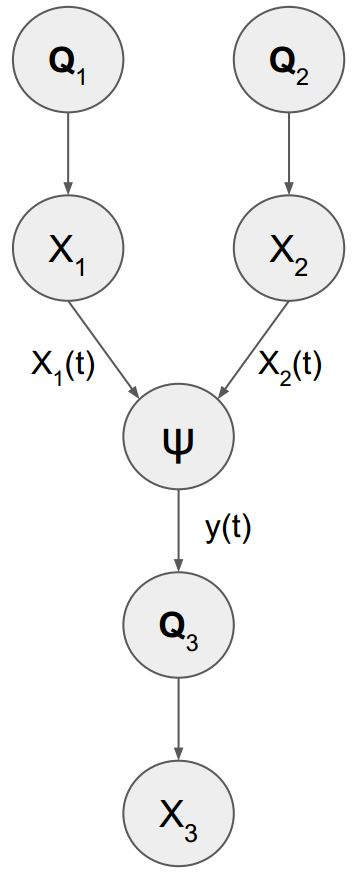
\includegraphics[width=0.75\linewidth]{figures/h_model}
%%	\column{.8\linewidth}
%	\begin{itemize}
%		\item While acting in the environment, the agent is assumed to have access to following parameters:
%		\begin{itemize}
%			\item Transition intensity matrices of the parents $ Q_{1} $ and $ Q_{2} $
%			\item Observation model $ \psi $
%			\item The optimal policy and $ \textbf{\textit{Q}}_{3} $
%		\end{itemize}
%		\item For the inference problem, the following parameters are given:
%		\begin{itemize}
%			\item Transition intensity matrices of the parents $ Q_{1} $ and $ Q_{2} $
%			\item The optimal policy and $ \textbf{\textit{Q}}_{3} $
%		\end{itemize}
%	\end{itemize}
%%\end{columns}
%\end{frame}


\begin{frame}{Exact Belief State Update}
\framesubtitle{Filtering CTMPs}
\begin{itemize}
%	\item Belief state is the probability distribution over state space given the observations
%	\begin{equation}
%	b(x_{1}, x_{2}; t) = P( X_{1}(t) = x_{1},  X_{2}(t) = x_{2}\mid y_{1}, ..., y_{t})
%	\end{equation}
%	\item Denote $ b(t) $, $ t \geq 0 $, as row vector with $ \left\lbrace b(x_{1}, x_{2};t)_{x_{i} \in \rchi_{i}}\right\rbrace  $.
\item Continuous-time solution of belief state through filtering for CTMPs, used as a baseline
%	\item Achieved by the inference of the posterior probability of $ X_P $, the joint process of the parent nodes
\item The posterior probability can be described by a system of ODEs
\begin{equation}
\frac{db(t)}{dt} = b(t)\ Q_P
\end{equation}
with the solution,
\begin{equation}
b(t) = b(0) \exp(tQ_P)
\end{equation}
where the initial condition $ b(0) $ is row vector with $ \left\lbrace b(x_P;t=0)\right\rbrace_{x_P \in \rchi_P} $ \cite{huang_pauleve_zechner_unger_hansen_koeppl_2016}.
\item $ Q_P $ is the joint transition intensity matrix of $ X_{1} $ and $ X_{2} $ and given by amalgamation operation between $ Q_{1} $ and  $ Q_{2} $ \cite{Nodelman1995}.
\begin{equation}
Q_P = Q_{1} * Q_{2}
\end{equation}
\end{itemize}
\end{frame}


\begin{frame}{Exact Belief State Update}
\framesubtitle{Filtering CTMPs}
\begin{itemize}
\item The belief update at discrete times of observation $ y_{L} = y(t_L) $ can be obtained as
\begin{align}
b(x_{P}; t_{L}) & = \operatorname{Pr}( X_P(t_{L}) = x_{P},\mid y_{1}, ..., y_{L}) \nonumber\\ & = \frac{\operatorname{Pr}(y_{1}, ..., y_{L}, X_P(t_{L}) = x_{P})}{\operatorname{Pr}(y_{1}, ..., y_{L})}  \nonumber\\ & = \frac{\operatorname{Pr}(y_{L} \mid y_{1}, ..., y_{L-1}, X_P(t_{L}) = x_{P})}{\operatorname{Pr}(y_{L} \mid y_{1}, ..., y_{L-1})} \frac{\operatorname{Pr}(y_{1}, ..., y_{L-1}, X_P(t_{L}) = x_{P})}{\operatorname{Pr}(y_{1}, ..., y_{L-1})}  \nonumber\\ & = Z_{L}^{-1} \ \operatorname{Pr}(y_{L} \mid X_P(t_{L})=x_{P})\ \operatorname{Pr}( X_P(t_{L}) = x_{P}\mid y_{1}, ..., y_{L-1})  \nonumber\\ & = Z_{L}^{-1}\ {p(y_{L} \mid x_{P})}\ {b(x_{P}; t_{L}^{-})}
\label{eq:b_jump}
\end{align}
where $ Z_{L} = \sum_{x_{P}\in \rchi_P} p(y_{L} \mid x_{P})\ b(x_{P}; t_{L}^{-}) $ is the normalization factor \cite{huang_pauleve_zechner_unger_hansen_koeppl_2016}.
\end{itemize}
\end{frame}


\begin{frame}{Belief State Update Using Particle Filter}
\begin{itemize}
\item The assumption that the complete information of parent dynamics is available is unrealistic.
\item The agent may rather have some prior beliefs over them. 
\item With exact update method, these parameters are assumed to be available for the inference as well. 
\item To simulate a more realistic model and be able to marginalize out these parameters from inference problem
\begin{itemize}
\item Replacing the exact belief update with marginal particle filter approximation
\end{itemize}
\end{itemize}
\end{frame}

\begin{frame}{Conditional Intensity Marginalization}
\framesubtitle{over $ Q_{1} $ and $ Q_{2} $}
\begin{itemize}
\item Given the priors and sample trajectory, the intensity matrices can be replaced by estimates. \cite{Studer2016}
\begin{itemize}
\item $Q_{n}$ with non-diagonal entries $ q^{n}_{i, j}\sim Gam(\alpha^{n}_{i, j}, \beta^{n}_{i, j}),\ \ n \in \left\lbrace 1,2\right\rbrace $
\item $X_{n}^{[0,T]}$ with summary statistics $ \Upsilon_{n}(x_i) $ and $ r_{n}(x_i,x_j) $, where $ \Upsilon_{n}(x_i) $ is the total time spent in state $ x_i $, $\ r_{n}(x_i,x_j) $ is the number of transitions from state $ x_i $ to state $ x_j $
\begin{align}
p(X_n^{[0,T]}  \mid Q) &=\left(\prod_{ i} q_{i}^{r_n(x_{i})} \exp \left(-q_{i} \Upsilon_n(x_{i})\right)\right)\left(\prod_{ i} \prod_{ j \neq i} \left(\frac{q_{i,j}}{q_{i}}\right)^{r_n(x_{i}, x_{j})}\right) \nonumber\\ & = \prod_{j \neq i}  \exp(-q_{i,j}\Upsilon_n(x_{i}))\ q_{i,j}^{r_n(x_{i},x_{j})}
\label{eq:lh_traj_homo}
\end{align}
\item Using Bayes' rule and the likelihood of trajectory in Eq.\autoref{eq:lh_traj_homo}, the estimates can be evaluated analytically as follows:
\begin{equation}
E\left[ q^{n}_{i,j} | X_n^{[0,T]}\right]=\frac{\alpha^{n}_{i,j}+r_{n}(x_i, x_j)}{\beta^{n}_{i, j}+\Upsilon_{n}(x_i)}
\label{eq:Q_estimate}
\end{equation}
\end{itemize}
\end{itemize}
\end{frame}

\begin{frame}{Marginal Particle Filter}
\begin{itemize}
%	\item Replacing the exact belief update with marginal particle filter approximation
%	\begin{itemize}
%		\item Removing the assumption that transition intensity matrices of $ X_{1} $ and $ X_{2} $ are available to agent $ X_{3} $
%		\item More realistic system
%	\end{itemize}
\item The particles to represent the belief state are drawn from a marginalized counterparts of parent processes \cite{Studer2016}.
\item With every new observation, the particles are propagated through the marginal process.
\begin{itemize}
\item The processing of the particles are done one after another. 
\item After each particle, the summary statistics are updated and the parameters are re-estimated using the Eq.\autoref{eq:Q_estimate}. 
\item The belief state is obtained as the distribution of states over the particles,
\begin{equation}
b(x_P; t) = \frac{1}{M} \sum_{m=1}^{M} \delta_{k_m(t), x_P}
\end{equation}
where $ M $ is the number of particles, $ k_i \in \textbf{k} $ is the set of particles, and $\delta$ is the Kronecker delta.
\end{itemize}
\end{itemize}
\end{frame}


\begin{frame}{Likelihood Model of the System}
\fontsize{9pt}{6}\selectfont
\begin{itemize}
\item Let $ S^{[0,T]} $ be a sample of trajectories in the dataset, such that $ S^{[0,T]} = \left\lbrace  X_{1}^{[0, T]}, X_{2}^{[0, T]}, X_{3}^{[0, T]} \right\rbrace   $, and the set of parameters to the system $  \theta = \left\lbrace  Q_{1}, Q_{2}, \textbf{\textit{Q}}_{3}, \pi, \psi \right\rbrace  $.
\vspace{5pt}
\item The likelihood of the sample $ S^{[0,T]} $ can be written as
\begin{align}
p(S^{[0,T]} \mid \theta ) & = p(X_{1}^{[0, T]}, X_{2}^{[0, T]}, X_{3}^{[0, T]} \mid Q_{1}, Q_{2}, \textbf{\textit{Q}}_{3}, \pi, \psi) \nonumber\\ & = p(X_{3}^{[0, T]} \mid X_{1}^{[0, T]}, X_{2}^{[0, T]}, \textbf{\textit{Q}}_{3}, \pi, \psi) \ p(X_{1}^{[0, T]}\mid Q_{1}) \ p(X_{2}^{[0, T]}\mid Q_{2}) \nonumber\\ & = p(X_{3}^{[0, T]}\mid Q_{3}^{[0, T]}) \ p(X_{1}^{[0, T]}\mid Q_{1}) \ p(X_{2}^{[0, T]}\mid Q_{2}) 
\end{align}
%	\vspace{-10pt}
\item Marginalized over $ Q_1 $ and $ Q_2 $
%	\vspace{-5pt}
\begin{align}
\begin{split}
p(S^{[0,T]} \mid \pi, \Phi ) = p(X_{3}^{[0, T]}\mid Q_{3}^{[0, T]}) \prod_{x_{1}\in\rchi_1} \frac{\beta_{x_{1}}^{\alpha_{x_{1}}}}{\Gamma(\alpha_{x_{1}})} \ (\Upsilon(x_{1})+\beta_{x_{1}})^{-r(x_{1})-\alpha_{x_{1}}}\ \Gamma(r(x_{1}) + \alpha_{x_{1}})  \\  \prod_{x_{2}\in\rchi_2} \frac{\beta_{x_{2}}^{\alpha_{x_{2}}}}{\Gamma(\alpha_{x_{2}})} \ (\Upsilon(x_{2})+\beta_{x_{2}})^{{-r(x_2)} - \alpha_{x_{2}}}\ \Gamma(r(x_2) + \alpha_{x_{2}})
\label{eq:Marg_llh_final}
\end{split}
\end{align}
%	where $ Q_{3}^{[0, T]} $ is a deterministic function of $X_{1}^{[0, T]}, X_{2}^{[0, T]}, Q_{1}, Q_{2}, \textbf{\textit{Q}}_{3}, \pi $ and $ \psi $.
\end{itemize}
\end{frame}


\begin{frame}{Simulation}
\framesubtitle{Sampling trajectories using Gillespie algorithm}
\vspace{12pt}
\begin{tabular}{cc}
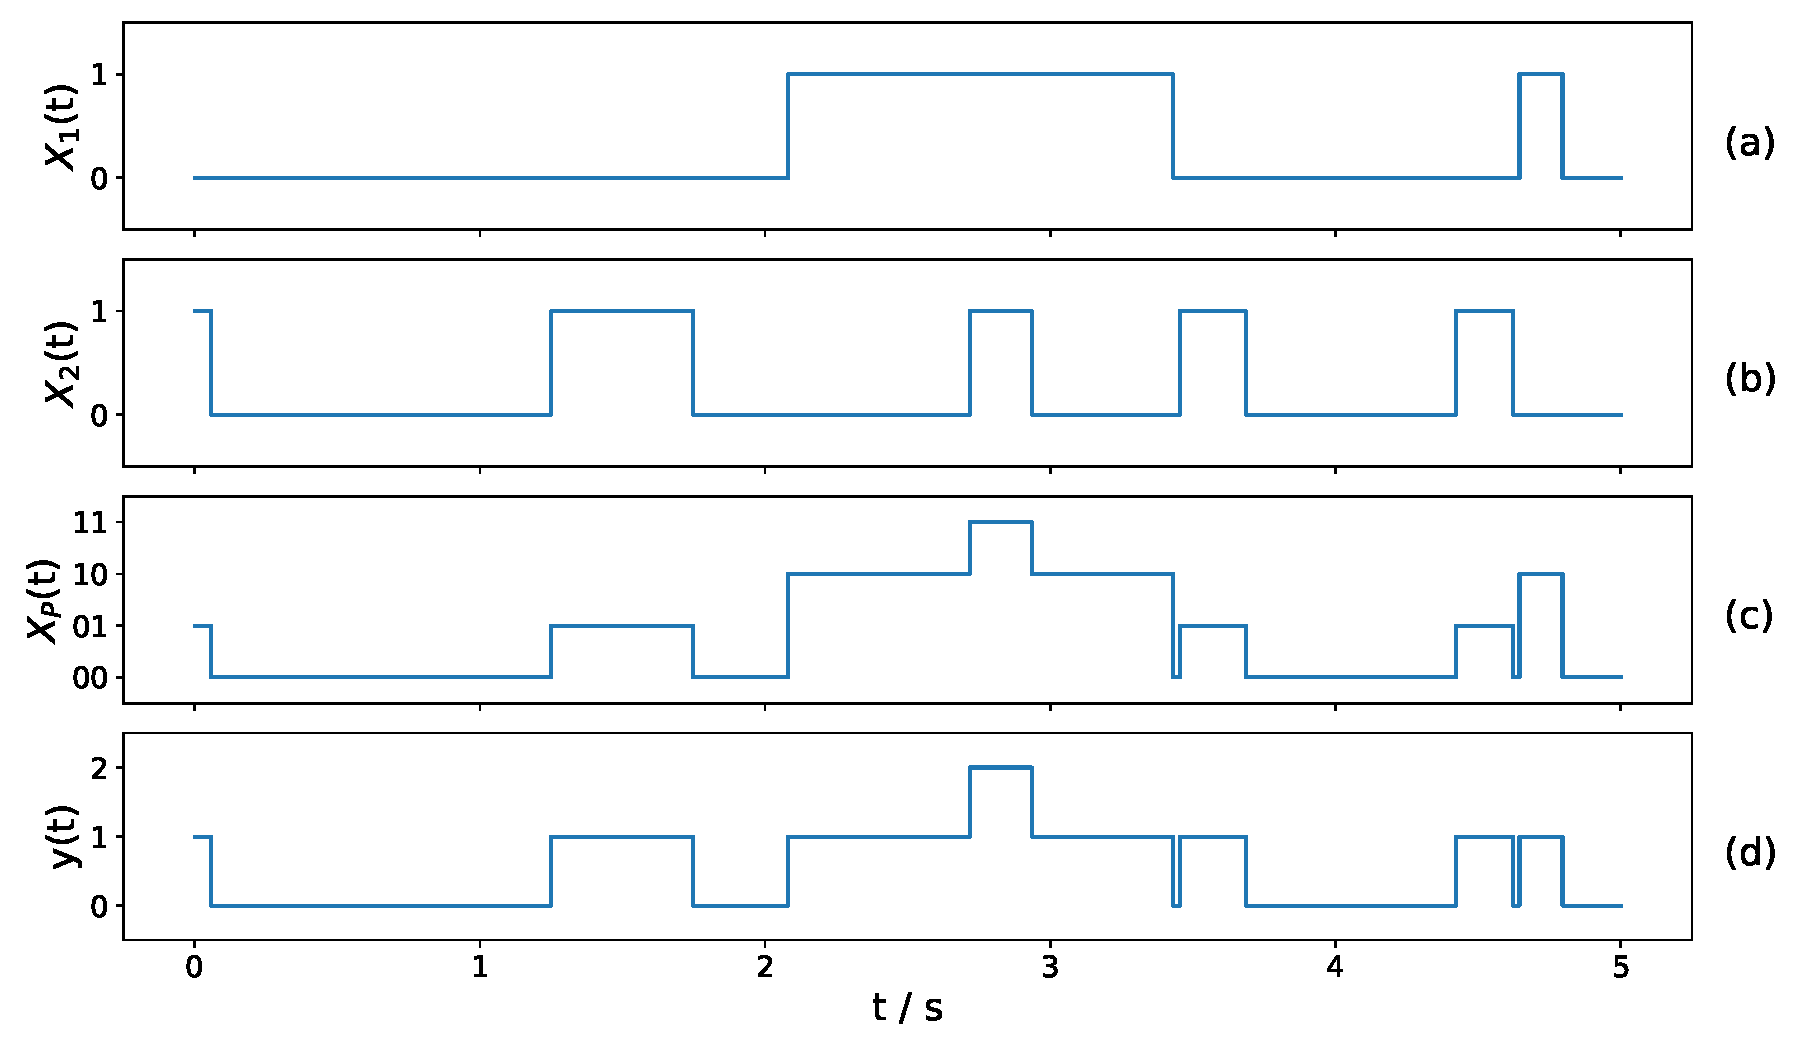
\includegraphics[height=0.6\textheight]{figures/parent_traj}
&
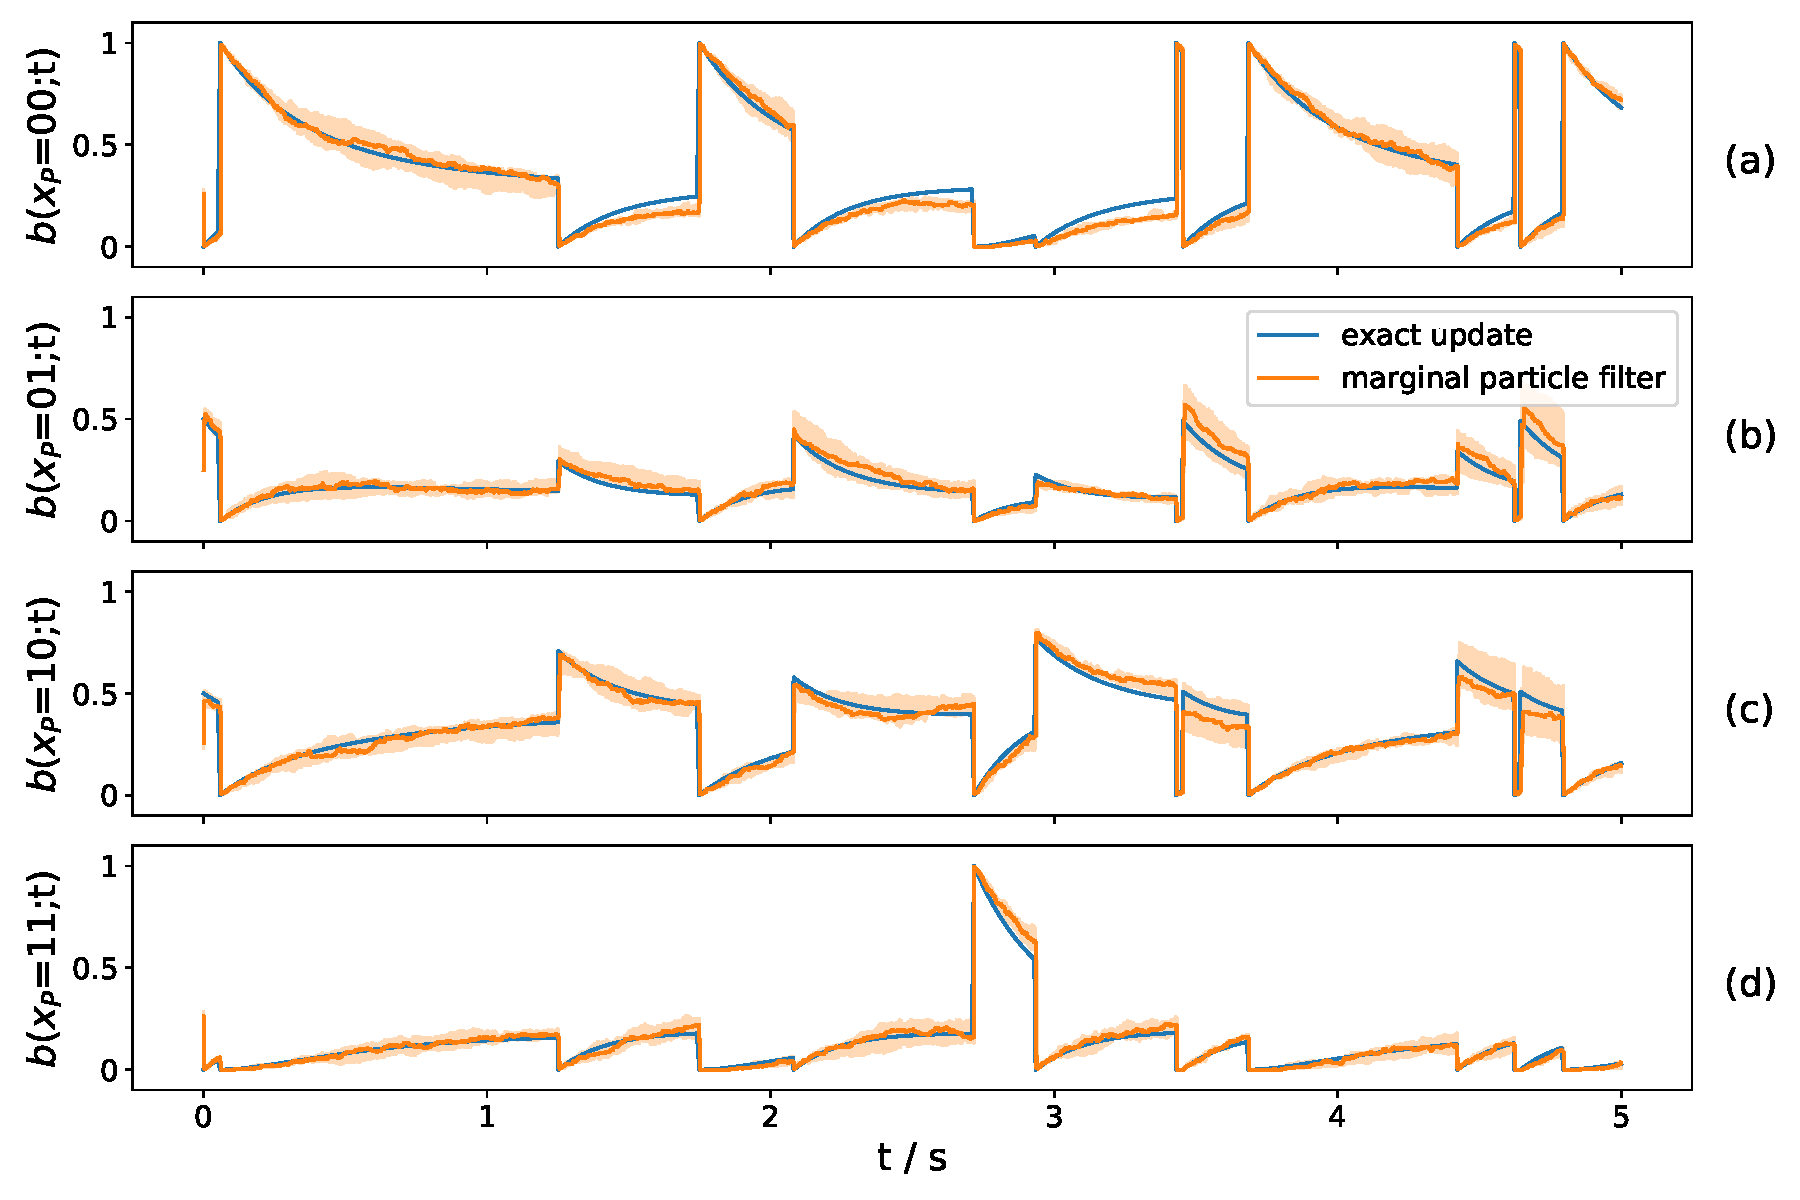
\includegraphics[height=0.6\textheight]{figures/belief_traj}
\end{tabular}
\end{frame}


\begin{frame}{Simulation}
\framesubtitle{Continued}
\centering
\begin{tabular}{cc}
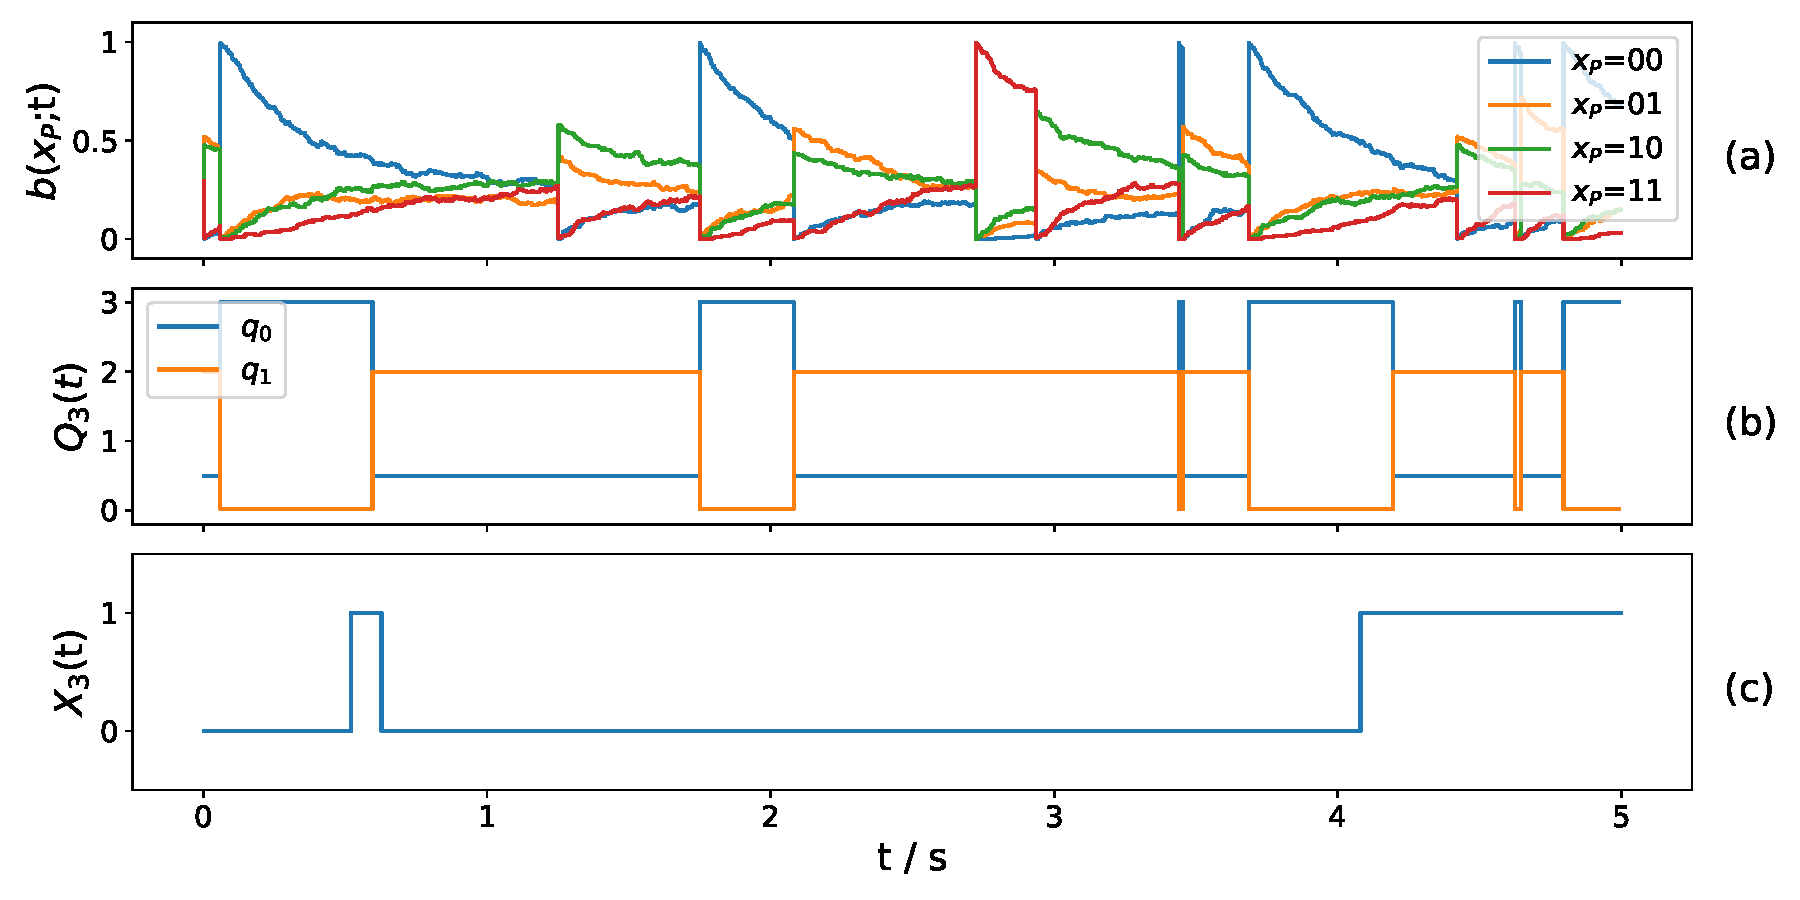
\includegraphics[height=0.7\textheight]{figures/q_traj}
\end{tabular}
\end{frame}


\begin{frame}{Limitation of Equivalence Classes}
\vspace{-5pt}
%\begin{columns}[T]
%	\column{0.5\textwidth}
%	\begin{itemize}
%		\item Identical effect on the belief state
%		\item Identical effect on the behaviour
%	\end{itemize}
%	\column{0.5\textwidth}
%	$ \psi_1 = 
%	\begin{bmatrix} \vspace{-3pt}
%	1 & 0 & 0 \\  \vspace{-3pt}
%	0 & 1 & 0 \\  \vspace{-3pt}
%	0 & 1 & 0 \\  \vspace{-2pt}
%	0 & 0 & 1
%	\end{bmatrix} $ $ \psi_2 = 
%	\begin{bmatrix} \vspace{-3pt}
%	0 & 0 & 1 \\  \vspace{-3pt}
%	0 & 1 & 0 \\  \vspace{-3pt}
%	0 & 1 & 0 \\  \vspace{-2pt}
%	1 & 0 & 0
%	\end{bmatrix} $
%\end{columns}
\begin{itemize}
\item Identical effect on the belief state
\item Identical effect on the behaviour
\end{itemize}
\vspace{+2pt}
\centering
\begin{tabular}{cc}
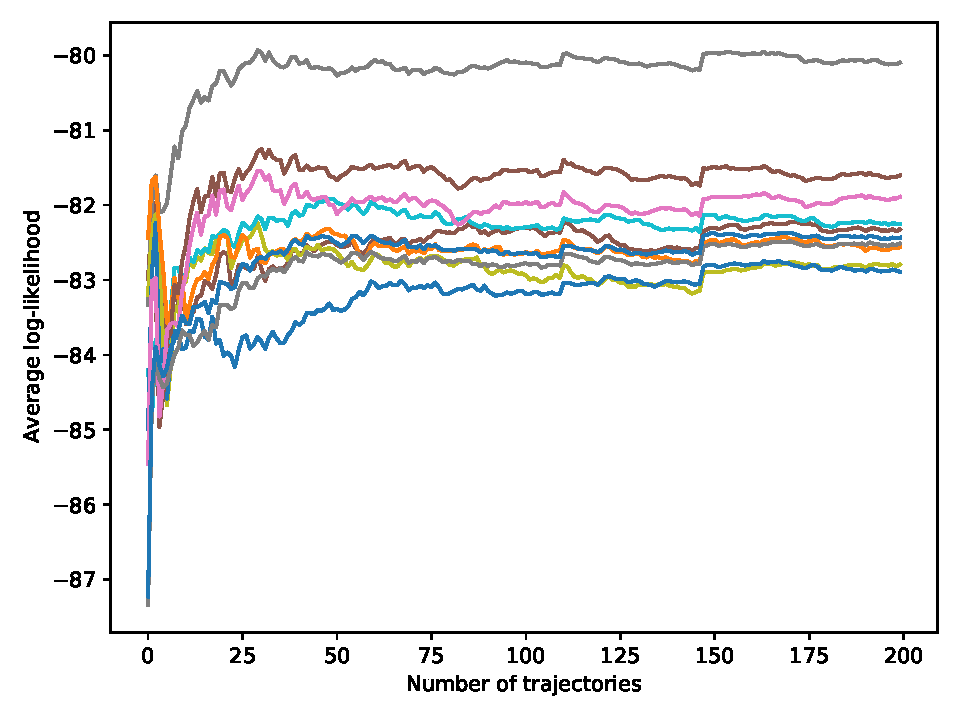
\includegraphics[height=0.6\textheight]{figures/llh_exactUpdate_81model}
&
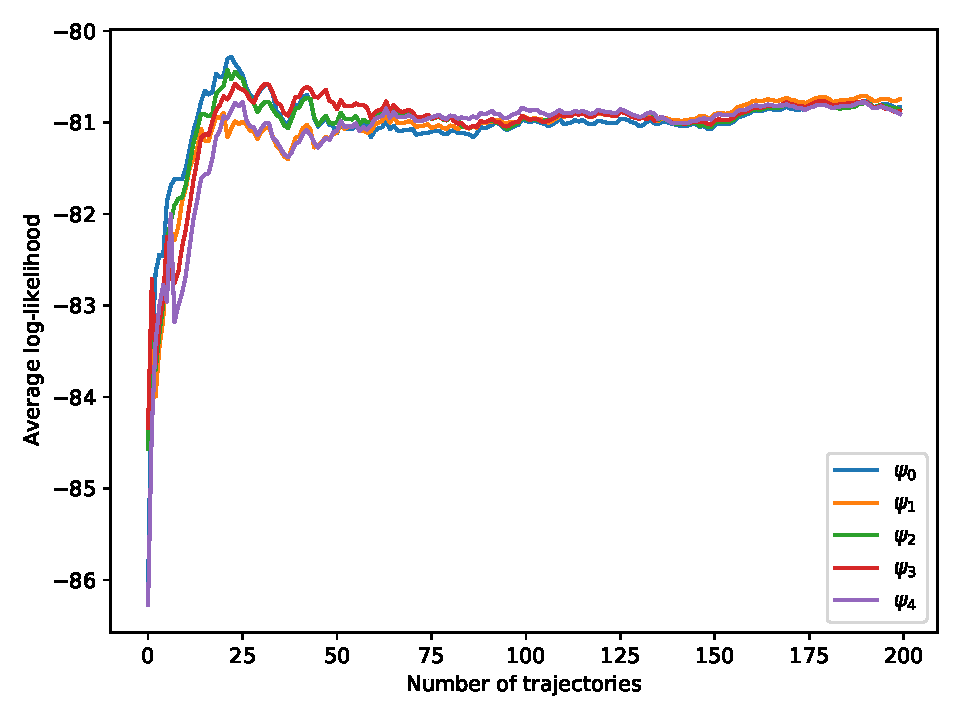
\includegraphics[height=0.6\textheight]{figures/llh_particleFilter_sameclass}
\end{tabular}
\end{frame}


\begin{frame}{Results}
\framesubtitle{Area under Receiver Operating Characteristic curve (AUROC)}
\begin{columns}[onlytextwidth,c]
\column{.5\linewidth}
\centering
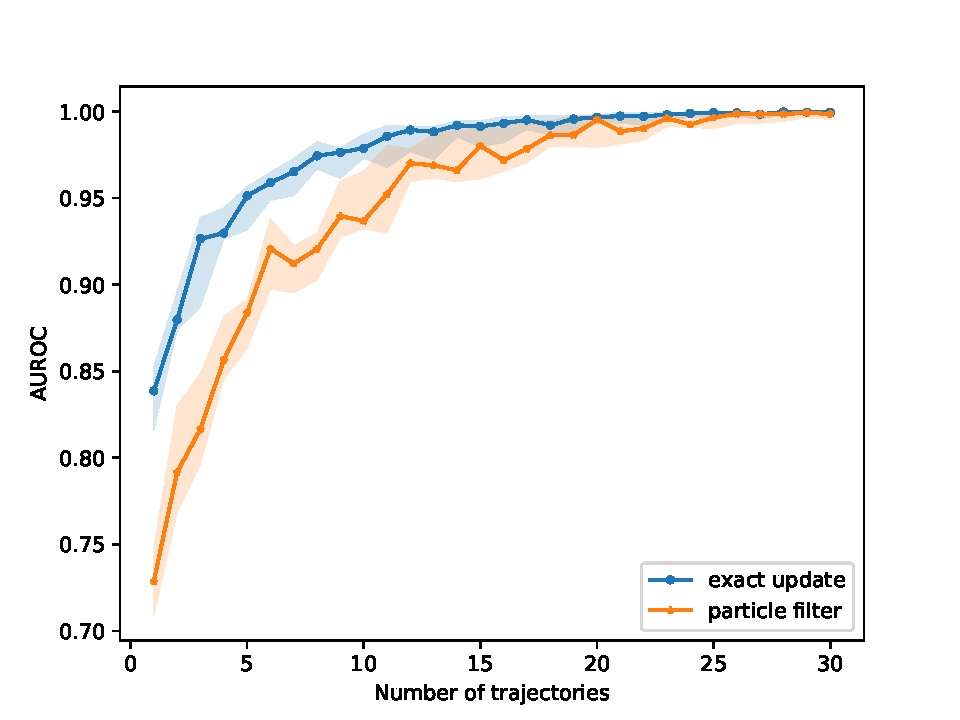
\includegraphics[width=\linewidth]{figures/AUROC_perc_0}
\column{.5\linewidth}
\begin{itemize}
\item The estimated likelihood values of each sample given an observation model as the score of the sample belonging to the corresponding class
\item Provided the classifier with increasing number of samples for inference
\item Through bootstrapping a given number of trajectories, and using the mean likelihood over the bootstrap batch as a new sample
%	\item The plots show the median with a line and the 25-75th percentile with the shaded area over 10 runs.
\end{itemize}
\end{columns}
\end{frame}


\begin{frame}{Results under Noise}
\framesubtitle{Area under Receiver Operating Characteristic curve (AUROC)}
\begin{columns}[onlytextwidth,c]
\column{.5\linewidth}
\centering
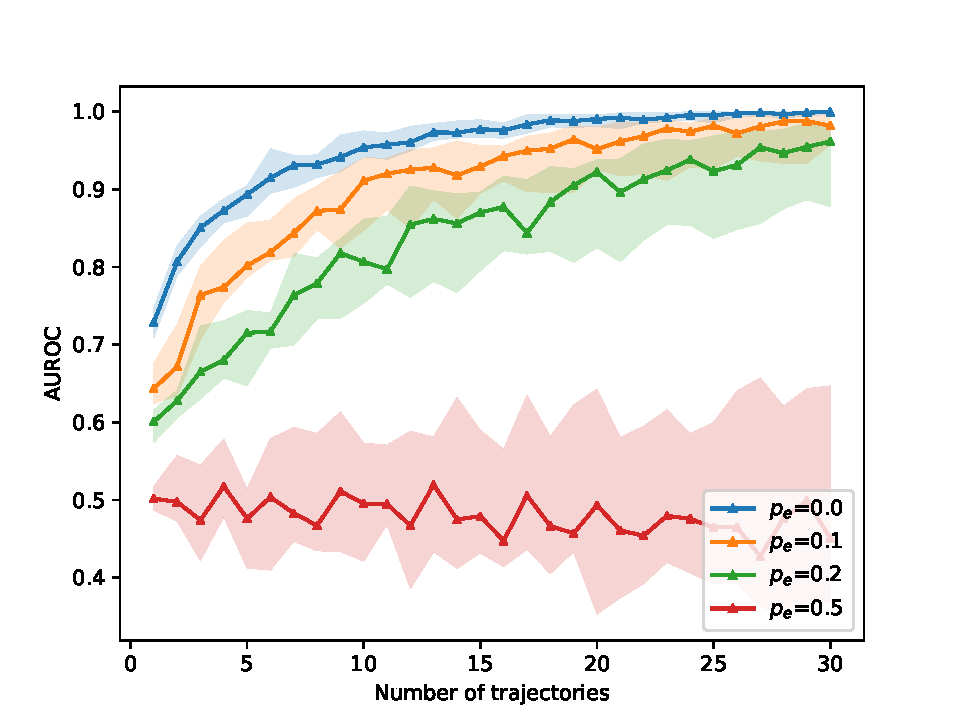
\includegraphics[width=\linewidth]{figures/error_AUROC_perc_0}
\column{.5\linewidth}
\begin{itemize}
\item $ p_e $ denotes the probability of producing erroneous observation.
\item Noisy observation model can be interpreted as a noisy communication channel with an error probability of $ p_e $.
\item The noise parameter is assumed to be available to the agent, i.e. it is not estimated.
\end{itemize}
\end{columns}
\end{frame}


\begin{frame}{Conclusion}
\begin{itemize}
\item A realistic system is achieved using particle filtering with marginalized CTBN. Given Gamma-priors of $ Q_1 $ and $ Q_2 $, the exact update method is well approximated by the marginal particle filter.
\item In classification, the marginal particle filter yields a slightly lower performance. Nevertheless, in both methods, as the number of samples increases, the metric approaches to 1.
\item The performance decreases as the noise introduced to the true observation model increases. With the increasing number of trajectories, the metric converges to 1, showing robustness.
\end{itemize}
\end{frame}


\begin{frame}{Outlook}
\vspace{-5pt}
\begin{itemize}
\item Eliminate the equivalence classes
\begin{itemize}
\item Joint inference of observation model and policy, i.e. function approximation
\end{itemize}
\item Application of the model and solution approach to a more complex
environment to evaluate the performance further
\begin{itemize}
\item Non-binary messages, more than two parent nodes etc.
\end{itemize}
\item Employing the method in different environments to get insights
into the interactions of agents and environments
\begin{itemize}
\item Inferring the communication protocols that lead
to the success or failure of the agents in Foerster's multi-step MNIST game \cite{Foerster2016}
\end{itemize}
\item Inference of observation model in an interactive multi-agent system
\end{itemize}
%\vspace{+.5cm}
\centering
\resizebox{.35\textwidth}{!}{
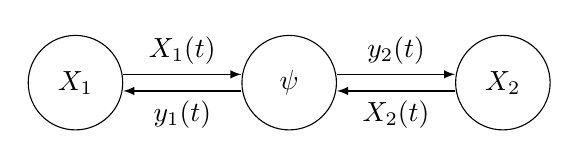
\begin{tikzpicture}
\tikzstyle{var} = [draw, circle, minimum size=1.2cm]
\tikzstyle{line} = [draw, -latex]

\node [var] (x1) {$X_1$};
\node [var, right=1.5cm of x1] (psi) {$\psi$};
\node [var, right=1.5cm of psi] (x2) {$X_2$};

\path [line] ([yshift=3pt]x1.east) -- node[pos=0.5, above] {$ X_1(t) $} ([yshift=3pt]psi.west) ;
\path [line] ([yshift=3pt]psi.east)  -- node[pos=0.5, above] {$ y_2(t) $} ([yshift=3pt]x2.west);
\path [line] ([yshift=-3pt]x2.west) -- node[pos=0.5, below] {$ X_2(t) $} ([yshift=-3pt]psi.east) ;
\path [line] ([yshift=-3pt]psi.west)  -- node[pos=0.5, below] {$ y_1(t) $} ([yshift=-3pt]x1.east);

\end{tikzpicture}
}
\end{frame}


\begin{frame}{References}
\vspace{-10pt}
\small
\bibliographystyle{ieeetr}
\bibliography{references}
\end{frame}


\begin{frame}[c]{}
\centering \Huge
Thank you!
\end{frame}


\begin{frame}[c]{}
\centering \Huge
Backup!
\end{frame}

\begin{frame}{Parameters}
\framesubtitle{Parameters}
\begin{columns}[T]
\column{.5\linewidth}
\begin{itemize}
\item Intensity matrices \vspace{+4pt}\\
$ Q_1 = 
\begin{bmatrix}
-1.117 & 1.117 \\
0.836 &  -0.836
\end{bmatrix} $\\
\vspace{+3pt}
$ Q_2 = 
\begin{bmatrix}
-1.1 & 1.1 \\
2.445 &  -2.445
\end{bmatrix}$\\
\vspace{+3pt}
$\textbf{\textit{Q}}_{3} = \left\lbrace 
\begin{bmatrix}\vspace{-2pt}
-0.5 & 0.5 \\\vspace{-2pt}
2 &  -2
\end{bmatrix}, 
\begin{bmatrix}\vspace{-2pt}
-3 & 3 \\\vspace{-2pt}
0.02 &  -0.02
\end{bmatrix} 
\right\rbrace $
\item Weights of the policy \vspace{+4pt} \\ $  w = \begin{bmatrix}0.02 & 0.833& 0.778& 0.87 \end{bmatrix}$
\end{itemize}
\column{.5\linewidth}
\begin{itemize}
\item Gamma priors for parent dynamics such that $ Q_{n} \sim \mathrm{Gam}(\boldsymbol{\alpha}^n, \boldsymbol{\beta}^n)$ for $n \in \left\lbrace 1,2\right\rbrace $, and $ \boldsymbol{\alpha}^n = [\alpha^n_0, \alpha^n_1] $ and $ \boldsymbol{\beta}^n = [\beta^n_0, \beta^n_1] $
\begin{align}
\boldsymbol{\alpha}^1 = [5,10] &\quad \boldsymbol{\beta}^1 = [5,20] \nonumber\\
\boldsymbol{\alpha}^2 = [10,10] &\quad \boldsymbol{\beta}^2 = [10,5] \nonumber
\end{align}
\item Number of particles $ M = 200 $
\end{itemize}
\end{columns}
\end{frame}


\begin{frame}{Markov Processes}
\begin{itemize}
\item Consider a homogenous Markov process X with values $ \rchi = \left\lbrace x_{0}, x_{1},..., x_{n}\right\rbrace  $. The transition intensity matrix Q of such process has the following form:
\begin{equation}
Q = 
\begin{bmatrix}
-q_{x_{0}} & q_{x_{0}x_{1}} & 	{\hdots}  & q_{x_{0}x_{n}} \\
q_{x_{1}x_{0}} & -q_{x_{1}} & 	{\hdots}  & q_{x_{1}x_{n}}  \\
{\vdots}  & 	{\vdots}  & 	{\ddots}  & {\hdots}  \\
q_{x_{n}x_{0}} &  q_{x_{n}x_{1}} &  {\hdots} & -q_{x_{n}}
\end{bmatrix}
\end{equation}
where $ q_{x} = \sum_{x' \neq x, x' \in \rchi} q_{xx'}$.
\item The amount of time that X stays in a transitioned state is exponentially distributed, and the probability density function of staying in a state x is given by \cite{Nodelman1995}
\begin{equation}
f(t) = q_{x}\ exp(-q_{x}t).
\end{equation}
\end{itemize}
\end{frame}


\begin{frame}{Likelihood Functions}
\framesubtitle{Homogenous continuous-time Markov process}
\fontsize{9pt}{6}\selectfont
\begin{itemize}
\item The likelihood of a single transition $ d = \left\langle x,t,x'\right\rangle $, where transition happens from $x$ to $x'$ after spending time amount of time t:
\begin{equation}
P(d  \mid Q) = \left( q_{x}\ exp(-q_{x}t) \right) \left( \frac{q_{xx'}}{q_{x}} \right)
\end{equation}
\item The likelihood of trajectory $X^{[0,T]}$ can be decomposed as a product of likelihood of single transitions.
\begin{align}
P(X^{[0,T]}  \mid Q) & = \left( \prod_{x}  q_{x}^{M[x]}\ exp(-q_{x}T[x]) \right) \left( \prod_{x} \prod_{x' \neq x}  \frac{q_{xx'}}{q_{x}}^{M[x,x']} \right) \nonumber\\ & = \prod_{x}  exp(-q_{x}T[x]) \prod_{x' \neq x}  q_{xx'}^{M[x,x']}
\label{homo_llh}
\end{align}
where $ T[x] $ is the total time spent in state x, $ M[x,x'] $ is the number of transitions from state x to state x', $ M[x] $ is total number of transitions leaving state x \cite{Nodelman2003}.
\end{itemize}
\end{frame}


\begin{frame}{Marginal Particle Filter}
\begin{itemize}
\vspace{-5pt}
\item Given a prior distribution over states, the particles are initialized $ \textbf{p}^{0} $.
\end{itemize}
\scalebox{1}{\begin{algorithm}[H]
\KwIn{Measurement data $ y_{k} $ at time $ t_{k} $, set of particles $ \textbf{p}^{k-1} $}
\KwResult{New set of particles $ \textbf{p}^{k} $, representing $ b(t_{k}) $}
\vspace{+4pt}
\begin{algorithmic}[1]
\FOR{$p_{m} \in \textbf{p}^{k-1}$}
\STATE {$p_{m} = \left\lbrace x_{m}, \textbf{T}_{m}, \textbf{M}_{m}\right\rbrace \leftarrow Propagate\ particle\ through\ marginal\ process\ model\ from\ t_{k-1}\ to\ t_{k}$ }
\STATE{$w_{m} \leftarrow p(y_{k} \mid X(t_{k})=x_{m}) $} 
\tcp*[h] {observation likelihood}
\ENDFOR
\STATE{$ w_{m} \leftarrow \frac{w_{m}}{\sum_{m} w_{m}}$} \tcp*[h]{normalize weights}
\FOR{$ p_{m} \in \textbf{p}_{k} $} 
\STATE{$ p_{m} \leftarrow Sample\ from\ p_{k}\ with\ probabilities\ w_{m}\ with\ replacement$}
\ENDFOR
\end{algorithmic}
\caption{Marginal particle filter\cite{Studer2016}}
\label{alg:seq}
\end{algorithm}}
\end{frame}


%%\begin{frame}{Likelihood model of the communication system}
%%\begin{itemize}
%%	\item Marginalizing the likelihood over $ Q_{1} $ and $ Q_{2} $:
%%	\begin{equation}
%%	\begin{split}
%%	P(\textit{D} \mid \pi, \phi ) & = 	\int \int P(\textit{D} \mid \theta ) \ P(Q_{1}) \ P(Q_{2}) \ dQ_{1}dQ_{2} \\ & = \int \int P(X_{3}^{[0, T]}\mid Q_{3}^{[0, T]}) \ P(X_{1}^{[0, T]}\mid Q_{1}) \ P(X_{2}^{[0, T]}\mid Q_{2}) \ P(Q_{1}) \ P(Q_{2})\ dQ_{1}d\textbf{Q}_{2} \\ & = P(X_{3}^{[0, T]}\mid Q_{3}^{[0, T]}) \int  P(X_{1}^{[0, T]}\mid Q_{1}) \ P(Q_{1}) \ dQ_{1} \int P(X_{2}^{[0, T]}\mid Q_{2})\ P(Q_{2})\ dQ_{2}
%%	\label{eq:Marg_llh}
%%	\end{split}
%%	\end{equation}
%%\end{itemize}
%%\end{frame}
%
%%
%%\begin{frame}{Likelihood model of the communication system}
%%\framesubtitle{Marginal probability of a trajectory of homogenous Markov Process}
%%\begin{itemize}
%%	\item 	Let X be a homogenous binary-valued Markov process.
%%	\item The transition intensity matrix Q can be written in the following form for convenience,
%%	\begin{equation}
%%		Q = 
%%		\begin{pmatrix}
%%		-q_{0} & q_{0} \\
%%		q_{1} & -q_{1}
%%		\end{pmatrix}
%%	\end{equation}
%%	where the transition intensities $ q_{0} $ and $ q_{1} $ are gamma-distributed with parameters $ \alpha_{0}$, $ \beta_{0} $ and $ \alpha_{1} $, $ \beta_{1} $, respectively.
%%\end{itemize}
%%\end{frame}
%
%
%%\begin{frame}[shrink=20]{Likelihood model of the communication system}
%%\framesubtitle{Marginal probability of a trajectory of homogenous Markov Process}
%%\vspace{-0.5cm}
%%	\begin{equation}
%%	\begin{split}
%%	P(X^{[0, T]}) & = \int  P(X^{[0, T]}\mid Q)P(Q) dQ \\ & = \int_{0}^{\infty} \left( \prod_{x} \exp(-q_{x}T_{x}) \prod_{x'} q_{xx'}^{M[x, x']}\right) \frac{\beta_{xx'}^{\alpha_{xx'}}{q_{xx'}^{\alpha_{xx'}-1}}\exp(-\beta_{xx'}q_{xx'})}{\Gamma(\alpha_{xx'})} \ dq_{xx'} \\ & = \prod_{x\in{0,1}}\int_{0}^{\infty} q_{x}^{M_{x}} \ \exp(-q_{x}T_{x}) \  \frac{\beta_{x}^{\alpha_{x}} \ q_{x}^{\alpha_{x}-1}\ \exp(-\beta_{x}q_{x})}{\Gamma(\alpha_{x})} \ dq_{x} \\ & = \prod_{x\in{0,1}} \frac{\beta_{x}^{\alpha_{x}}}{\Gamma(\alpha_{x})} \int_{0}^{\infty} q_{x}^{M_{x} + \alpha_{x} -1} \ \exp(-q_{x}(T_{x}+\beta_{x})) \ dq_{x} \\ & = \prod_{x\in{0,1}} \frac{\beta_{x}^{\alpha_{x}}}{\Gamma(\alpha_{x})} \left( -(T_{x}+\beta_{x})^{M_{x} + \alpha_{x}}\ \Gamma(M_{x} + \alpha_{x}, \ q_{x}(T_{x}+\beta_{x})) \right) \Big|_0^\infty  \\ & = \prod_{x\in{0,1}} \frac{\beta_{x}^{\alpha_{x}}}{\Gamma(\alpha_{x})} \left( (T_{x}+\beta_{x})^{M_{x} + \alpha_{x}}\ \Gamma(M_{x} + \alpha_{x}) \right)
%%	\label{eq:Marg_traj}
%%	\end{split}
%%	\end{equation}
%%	where $ T_{x} $, the amount of time spent in state x, $ M[x,x'] $ the number of transitions from state x to x' and  $ M[x] = \sum_{x\neq x'}M[x,x'] $.
%%\end{frame}
%
%%
%%\begin{frame}{Likelihood model}
%%\framesubtitle{Overall system}
%%\begin{itemize}
%%	\item Plugging Eq.\ref{eq:Marg_traj} in Eq.\ref{eq:Marg_llh} for both $ X_{1} $ and $ X_{2} $:
%%	\begin{align}
%%	\begin{split}
%%	P(\textit{D} \mid \pi, \phi ) = P(X_{3}^{[0, T]}\mid Q_{3}^{[0, T]}) \prod_{x_{1}\in{0,1}} \frac{\beta_{x_{1}}^{\alpha_{x_{1}}}}{\Gamma(\alpha_{x_{1}})} \ (T_{x_{1}}+\beta_{x_{1}})^{M_{x_{1}} + \alpha_{x_{1}}}\ \Gamma(M_{x_{1}} + \alpha_{x_{1}})  \\  \prod_{x_{2}\in{0,1}} \frac{\beta_{x_{2}}^{\alpha_{x_{2}}}}{\Gamma(\alpha_{x_{2}})} \ (T_{x_{2}}+\beta_{x_{2}})^{M_{x_{2}} + \alpha_{x_{2}}}\ \Gamma(M_{x_{2}} + \alpha_{x_{2}})
%%	\label{eq:Marg_llh_final}
%%	\end{split}
%%	\end{align}
%%\end{itemize}
%%\end{frame}
%%

%\begin{frame}{Exact Belief State Update}
%\framesubtitle{Filtering CTMPs}
%\begin{itemize}
%	\item The belief update at discrete times of observation $ y_{t} $
%	\begin{align}
%	b(x_{1}, x_{2}; t) & = P( X_{1}(t) = x_{1},  X_{2}(t) = x_{2}\mid y_{1}, ..., y_{t}) \nonumber\\ & = \frac{P(y_{1}, ..., y_{t}, X_{1}(t) = x_{1},  X_{2}(t) = x_{2})}{P(y_{1}, ..., y_{t})}  \nonumber\\ & = \frac{P(y_{t} \mid y_{1}, ..., y_{t-1}, X_{1}(t) = x_{1},  X_{2}(t) = x_{2})}{P(y_{t} \mid y_{1}, ..., y_{t-1})} \frac{P(y_{1}, ..., y_{t-1}, X_{1}(t) = x_{1},  X_{2}(t) = x_{2})}{P(y_{1}, ..., y_{t-1})}  \nonumber\\ & = Z_{t}^{-1} \ P(y_{t} \mid x_{1}, x_{2})\ P( X_{1}(t) = x_{1},  X_{2}(t) = x_{2}\mid y_{1}, ..., y_{t-1})  \nonumber\\ & = Z_{t}^{-1}\ \textcolor[rgb]{0.16,0.32,0.75}{P(y_{t} \mid x_{1}, x_{2})}\ \textcolor[rgb]{0.8,0,0}{b(x_{1}, x_{2}; t^{-})}
%	\end{align}
%	where $ Z_{t} = \sum_{x_{1}, x_{2}\in X} P(y_{t} \mid x_{1}, x_{2})\ b(x_{1}, x_{2}; t^{-}) $ is the normalization factor \cite{huang_pauleve_zechner_unger_hansen_koeppl_2016}.
%\end{itemize}
%\end{frame}


\end{document}